\documentclass{article}
\usepackage{tikz}
\usetikzlibrary{shapes,positioning,trees}

\tikzset{
  basic/.style = {draw, rectangle},
  every node/.style = {basic, rounded corners=2pt, thin, align=center, fill=purple!30},
}

\begin{document}
\pagestyle{empty}

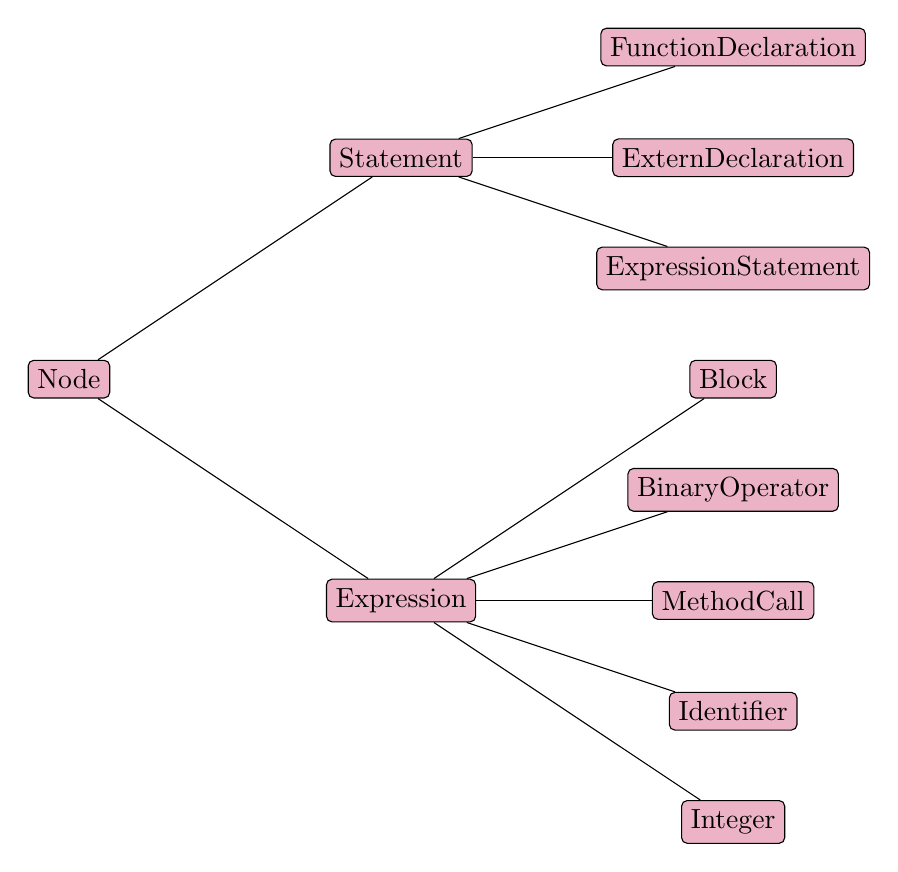
\begin{tikzpicture}[
  grow = right,
  edge from parent/.style = {draw},
  level 1/.style={sibling distance = 16em},
  level 2/.style={sibling distance = 4em},
  level distance = 12em,
 ]
 
 \node {Node}
 child {node[level 1] {Expression}
   child {node[level 2] {Integer}}
   child {node[level 2] {Identifier}}
   child {node[level 2] {MethodCall}}
   child {node[level 2] {BinaryOperator}}
   child {node[level 2] {Block}}
  }
 child {node[level 1] {Statement}
   child {node[level 2] {ExpressionStatement}}
   child {node[level 2] {ExternDeclaration}}
   child {node[level 2] {FunctionDeclaration}}
  };
 
\end{tikzpicture}
\end{document}
